\scanpage{16}
\mspage{13}

à la somme directe de ses comp. connexes. Si $\mathcal X=(L,\underset{\substack{\cap\\\mathcal P(L)}}{S},\delta)$ est régulier, \inserted{et} ses comp. connexes le sont. \unsure{Donc} l'étude des modèles $\mathcal X$ réguliers \deleted{\unsure{est}} revient à celle des modèles réguliers connexes.

Soit $(L,\underset{\substack{\cap\\\mathcal P(L)}}{S},\delta:\deleted{\unsure{\delta}}S\unsure{\longrightarrow|-}\mathcal P_2(L))$ un modèle régulier connexe. On va définir un système transitif de bij. entre les $\delta I$ $(I\in S)$. et entre les $B_x$ $(x\in L)$ et entre

\deleted{Soient $I,J\in S$}

les uns et les autres. \deleted{Soit $x\in L,\ y\in L$.}

\figure{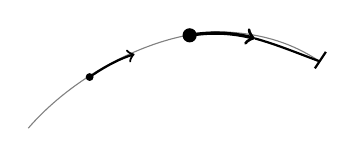
\begin{tikzpicture}[x=1cm,y=1cm]
\draw[gray,thin] (0,0) .. controls (0.65,0.75) and (1.75,1.27) .. (2.55,1.22) .. controls (3,1.19) and (3.35,1.08) .. (3.7,0.85);
\fill (0.78,0.65) circle (0.05);
\draw[thick,->] (0.78,0.65) .. controls (0.98,0.79) and (1.18,0.89) .. (1.35,0.94);
\fill (2.05,1.18) circle (0.09);
\draw[very thick,->] (2.05,1.18) .. controls (2.34,1.23) and (2.61,1.21) .. (2.88,1.14);
\draw[thick] (2.88,1.14) .. controls (3.17,1.06) and (3.48,0.93) .. (3.7,0.85);
\draw[thick] (3.64,0.76)--(3.78,0.97);
\end{tikzpicture}}

\uline{Th} On peut trouver, \inserted{de façon unique,} un syst. transitif d'iso entre les $\delta I$ $(I\in S)$ avec un quotient $\omega_S$, et un syst. transitif d'iso entre les $B_x$ $(x\in L)$, avec un quotient $\omega_L$, et une bijection $\omega_S\simeq\omega_L$ (soit $\underline{\omega}$ le quotient) -- donc un système d'iso $\underline{\omega}\simeq\delta I$, $\underline{\omega}\simeq B_x$, de façon que les conditions

\mspage{15}

% the paper's watermark (EXTRA STRONG), not his text
% the paper's watermark (EXTRA STRONG), not his text
